\subsection{Backend}
Das Backend besteht aus mehrere Paketen und ist wie folgt aufgebaut:
\begin{figure}[H]
	\centering
	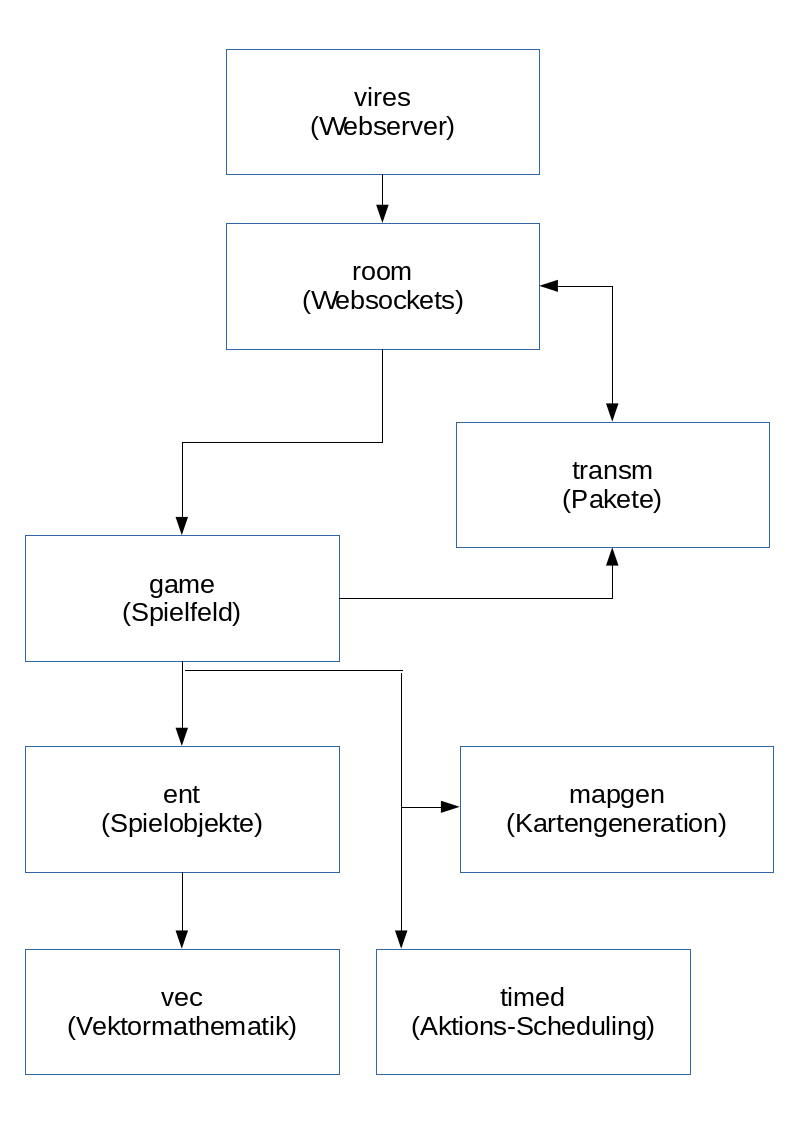
\includegraphics[width=0.6\textwidth]{Architektur.png}
	\caption{Paketaufbau des Backends}
\end{figure}
Die Bedeutung der einzelnen Pakete und wichtige Algorithmen werden im Folgenden erklärt.

\subsubsection{vires}
\verb+vires+ ist das Main-Package des Programms und kümmert sich um die Verwaltung des Webservers von \vires. \\
Wird eine GET-Anfrage auf einen Link ausgeführt, der eine Room-ID enthält (z.B. \url{http://localhost/1234}), so wird eine Template für den Raum, welche mit der Room-ID kompiliert wird, an den User gesendet. \\
Die kompilierte Template öffnet hieraufhin eine Websocket-Verbindung zu \verb+/<roomid>/c+. \\
Der Handler für \verb+/<roomid>/c+ eröffnet dann auch serverseitig die Websocket-Verbindung und übergibt die Verbindung an die jeweilige \verb+room+-Instanz.

\subsubsection{room}
\verb+room+ verwaltet die Websocket-Verbindungen eines Rooms. Verbindet sich der erste User mit dem Room, so wird der Room erstellt. \\
Alle Operationen eines Rooms werden von einer Monitor-Goroutine verwaltet, welche den Zugriff auf alle Zustände des Rooms synchronisiert. \\
Insgesamt verwaltet die Monitor-Goroutine Spielerverbindungen, Matches, Pakete von und an Nutzer und Pakete vom Spiel. \\
Genauere Informationen über Monitor-Goroutines können unter \verb+MONITOR_GOROUTINE_REF_HIER_EINFÜGEN+ gefunden werden. \\
Wird eine Websocket-Verbindung zu dem Room hinzugefügt, so werden für diese Verbindung eine Reader- und eine Writer-Goroutine gestartet. 

\subsubsection{game}
\verb+game+ verwaltet eine Spielinstanz. Eine Spielinstanz wird als Spielfeld ausgedrückt, welches sich um alle Spieloperationen kümmert, welche das gesamte Spielfeld erfordern. \\
Der \vires-Server verfolgt einen anderen Ansatz als die meisten Serverapplikationen von Spielen: 
Anstatt innerhalb eines Game-Loops zu überprüfen, ob bestimmte Bedingungen erfüllt sind,
werden alle Aktionen vorberechnet und mittels Timern und einem Scheduler verzögert, bis die Aktion ausgeführt werden soll. \\
\vires\ ist langsam und der Server soll in der Lage sein, sehr viele Matches gleichzeitig auszuführen. 
Würde der Server für jedes Match Game-Loops verwenden, so wäre entweder die Bearbeitungszeit sehr schlecht oder eine hohe
Überprüfungsfrequenz würde Serverleistung verschwenden. \\
\verb+room+ kommuniziert mit \verb+game+, indem es Methoden von \verb+game+ aufruft, wenn Nutzereingaben erfolgen. \\
\verb+game+ kommuniziert mit \verb+room+, indem es Nachrichten über \verb+transm+ nach \verb+room+ schickt, wenn das Spiel den Spielern etwas mitteilen muss. \\
Insgesamt verwaltet \verb+game+ Movements, Collisions und Conflicts. Jede Aktion auf dem Spielfeld wird über den \verb+timed+-Scheduler
ausgeführt, um Zustandszugriffe vom Spiel und von Nutzern zu synchronisieren. \\
Wird ein Movement gestartet, so wird zuerst geprüft, ob das Movement erlaubt ist. Ist es erlaubt, so wird ein Movement erzeugt, 
ein Conflict am Zeitpunkt des Conflicts für die Target-Cell geschedulet und mit jedem anderen Movement geprüft, ob es eine Collision gibt. \\
Gibt es eine Collision, so wird die Collision beiden kollidierenden Movements hinzugefügt und für den Zeitpunkt der Collision geschedulet.
Tritt der Conflict auf, so wird das Movement entfernt, die Anzahl an Moving Vires je nach Art des Conflicts der Cell hinzugefügt oder der Cell abgezogen,
überprüft, ob die Cell den Besitzer gewechselt hat, überprüft, ob der Besitzer tot ist und geprüft, ob ein Spieler das Match gewonnen hat. \\
Tritt eine Collision auf, so kämpfen die Movements miteinander oder vereinen sich je nach Art der Collision.
Hieraufhin werden alle Collisions beider Movements entfernt und neu berechnet, da die Anzahl an Moving Vires die Größe und die Geschwindigkeit beeinflusst und sich somit auch die Situation für zukünftige Collisions ändert.
Stirbt eines der Movements, so wird der Conflict für das jeweilige Movement entfernt. \\
Es wird also insgesamt beim Erzeugen eines Movements berechnet, welche Collisions nach der aktuellen Situation auftreten können, 
verändert sich aber die Situation auf dem Spielfeld, so werden erst zum Zeitpunkt der Situationsveränderung die jeweiligen Änderungen 
an den anliegenden Movements vorgenommen. \\
Beim Erzeugen der Movements wird zuerst nur davon ausgegangen, dass die auftretenden Collisions alle mit der Startgröße und der Startgeschwindigkeit stattfinden. \\
Hieraus ergibt sich, dass lediglich die anliegenden Movements verändert werden müssen, und nicht rekursiv alle Movements die nach der aktuellen Collision stattfinden. \\
Das folgende Szenario ist anzunehmen:
\begin{figure}[H]
	\centering
	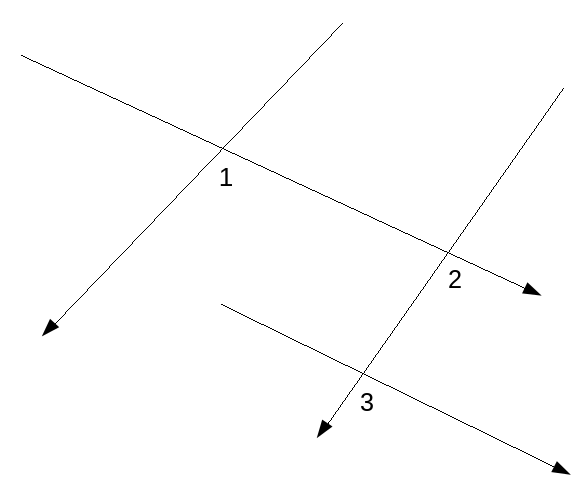
\includegraphics[width=0.8\textwidth]{Collision.png}
\end{figure}
Movements werden als Pfeile dargestellt. Alle vier Movements werden zeitnah hinzugefügt. Beim Hinzufügen aller Movements wird bestimmt, dass mit der Startgeschwindigkeit und dem Startradius des Movements die drei Collisions 1, 2 und 3 in der genannten Reihenfolge stattfinden. Für jede Collision wird für den Zeitpunkt der Collision nach Startgeschwindigkeit und Startradius eine Collision geschedulet. \\
Zuerst tritt Collision 1 auf. Hieraus ergeben sich drei Fälle für Collision 2:
\begin{enumerate}
	\item Collision 2 findet nicht mehr statt (Das Movement wurde zerstört)
	\item Collision 2 findet schneller statt (Das Movement ist kleiner geworden)
	\item Collision 2 finden langsamer statt (Das Movement hat sich mit dem anderen Movement vereint)
\end{enumerate}
In der Folge auf Collision 1 werden alle Collisions der beiden anliegenden Movements aktualisiert. \\
\begin{itemize}
	\item Tritt Fall 1 ein, so wird Collision 2 entfernt und Collision 3 findet wie erwartet mit Startgeschwindigkeit und Startradius statt
	\item Tritt Fall 2 oder 3 ein, so wird Collision 2 stattfinden, und hierbei die Geschwindigkeit und der Radius während Collision 2 angepasst
\end{itemize}
Es ist also nur nötig, die Collisions, welche mit den kollidierenden Movements verbunden sind, zu aktualisieren, da Fall 1 vom Default abgedeckt wird, während Fall 2 und Fall 3 in dem jeweiligen Zeitpunkt bestimmt werden können. Würde Fall 1 nicht vom Default abgedeckt werden, so müsste man rekursiv alle Collisions aktualisieren, die direkt und indirekt mit den betroffenen Movements verbunden sind, da die Kollisionszeit von Collision 3 aktualisiert werden müsste, und somit auch für alle damit verbundenen Movements. \\

Dieser Algorithmus verhält sich gegenüber einigen Alternativen wie folgt:
\begin{itemize}
	\item Feststellen der nächsten Collision beim Hinzufügen jedes Movements und bei jeder Collision 
	($T(\frac{n \cdot (n - 1)}{2})$, bzw. $\mathcal{O}(n^2)$, beim Hinzufügen von Movements und bei Collisions)
	\item Rekursive Erfassung der Collisions beim Hinzufügen eines Movements und beim Stattfinden einer Collision 
	($T(\frac{n \cdot (n - 1)}{2})$, bzw. $\mathcal{O}(n^2)$, beim Hinzufügen von Movements und bei Collisions)
	\item Rekursive Erfassung der kompletten Spielsituation beim Hinzufügen eines Movements 
	($T(\frac{n \cdot (n - 1)}{2})$, bzw. $\mathcal{O}(n^2)$, beim Hinzufügen eines Movements)
	\item Einfache Erfassung der anliegenden Movements bei der Collision und Annahme, dass alle Collisions unverändert stattfinden beim Hinzufügen eines Movements 
	($T(n)$, bzw.  $\mathcal{O}(n)$ beim Hinzufügen eines Movements und bei Collisions)
\end{itemize}
Die Zustandsraumkomplexität des Algorithmus ist $\mathcal{O}(n^2)$, da sich für jedes Movement bis n Movements gemerkt werden müssen.
Es wäre möglich, die Zustandsraumkomplexität weiterhin auf $\mathcal{O}(n)$ zu reduzieren, indem man sich lediglich die nächste Collision eines Movements anstatt alle Collisions eines Movements merkt, was allerdings in anderen Bereichen für größere Kosten sorgen würde und schwerer umzusetzen ist, als die aktuelle Version des Algorithmus.